% step-refinement.tex

\documentclass[tikz]{standalone}
\usetikzlibrary{positioning, arrows.meta}

\newcommand{\red}[1]{\textcolor{red}{#1}}

\begin{document}
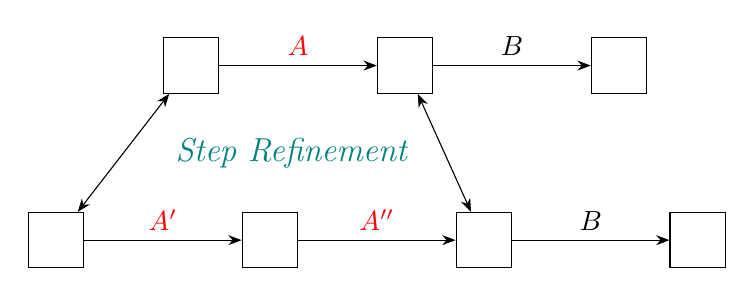
\begin{tikzpicture}[state/.style = {draw, rectangle, minimum size = 20pt},
  node distance = 1.5cm and 2.0cm, >=Stealth] 
  \node (1) [state] {};
  \node (2) [state, right = of 1] {};
  \node (3) [state, right = of 2] {};
  \path (1) edge[->] node [above] {\red{$A$}} (2)
	(2) edge[->] node [above] {$B$} (3);

  \node (11) [state, below left = 1.5cm and 1.0cm of 1] {};
  \node (22) [state, right = of 11] {};
  \node (33) [state, right = of 22] {};
  \node (44) [state, right = of 33] {};
  \path (11) edge[->] node [above] {\red{$A'$}} (22)
	(22) edge[->] node [above] {\red{$A''$}} (33)
	(33) edge[->] node [above] {$B$} (44);

  \draw [<->] (1) to (11);

  \draw [<->] (2) to node [align = center, left = 10pt] {\textcolor{teal}{\it \large Step Refinement}} (33);
\end{tikzpicture}
\end{document}
